%\graphicspath{{~/Pictures/Screenshots/}}
\graphicspath{{~/Documents/MobAppDev/fifth/img}}
\section*{\LARGE{Цель практической работы}}
\addcontentsline{toc}{section}{Цель практической работы}
Создать примеры, реализующие основные элементы управления:

\begin{itemize}
	\item Элемент TextView и его атрибуты. Установка элемента в коде.
		Используя атрибут android:autoLink вывести на экран ссылку и телефон;
	\item Элемент EditText и его атрибуты. Используя атрибуты
		android:hint и android:inputType задать текст, который будет
		отображаться в качестве подсказки, если элемент EditText пуст
		и клавиатуру для ввода. Реализовать два поля.
		Первое поле --- однострочное, а второе --- многострочное.
		Введенные символы в первом поле --- отображаются во втором;
	\item Элемент Button и его атрибуты. Реализовать на экране кнопку с
		надписью “Ввод”. После нажатия на кнопку выводится текст из первого
		поля во второе. Реализовать аналогичный пример полностью в коде;
	\item Класс Toast. Всплывающие окна. Toast можно использовать
		только в коде java. Реализуйте это, используя метод Toast.makeText().
		В качестве времени показа окна можете использовать целочисленное
		значение - колическо миллисекунд или встроенные константы
		\verb|Toast.LENGTH_LONG| (2000 миллисекунд)
		и \verb|Toast.LENGTH_SHORT| (2000 миллисекунд).
		Используйте метод setGravity для указания, в какой части
		контейнера надо позиционировать Toast;
	\item Элемент Snackbar. Реализуйте пример с помощью метода make().
		Прикрепление обработчика события. Реализуйте пример с помощью метода
		setAction().Реализуйте пример с настройкой визуального вида;
	\item Элементы Checkbox. Реализуйте пример с несколькими
		флажками которые могут находиться в отмеченном и неотмеченном
		состоянии;
	\item Слушатель OnCheckedChangeListener. Реализуйте пример с
		помощью метода onCheckedChanged;
	\item Элемент ToggleButton. Реализуйте пример с помощью атрибутов
		android:textOn и android:textOff. Реализуйте пример создания элемента
		ToggleButton в коде java;
	\item Класс RadioButton Реализуйте пример;
	\item Элемент DatePicker. Реализуйте пример;
	\item Элемент TimePicker Реализуйте пример;
	\item Элемент SeekBar (Ползунок). Реализуйте пример.
\end{itemize}

\clearpage

\section*{\LARGE{Выполнение практической работы}}
\addcontentsline{toc}{section}{Выполнение практической работы}

\section{Элемент TextView}
Для простого вывода текста на экран предназначен элемент TextView. 
Он просто отображает текст без возможности его редактирования. 
Некоторые его основные атрибуты:

\begin{itemize}
	\item \texttt{android:text}: устанавливает текст элемента;
	\item \texttt{android:textSize}: устанавливает высоту текста,
		в качестве единиц измерения для указания высоты используются sp;
	\item \texttt{android:background}: задает фоновый цвет элемента в виде
		цвета в шестнадцатиричной записи или в виде цветового ресурса;
	\item \texttt{android:textColor}: задает цвет текста;
	\item \texttt{android:textAllCaps}: при значении true делает все символы
		в тексте заглавными;
	\item \texttt{android:textDirection}: устанавливает направление текста.
		По умолчанию используется направление слева направо, но с помощью
		значения rtl можно установить направление справо налево;
	\item \texttt{android:textAlignment}: задает выравнивание текста;
	\item \texttt{ndroid:fontFamily}: устанавливает тип шрифта.
\end{itemize}

Чтобы вывести на экран какую-нибудь ссылку, либо телефон,
по нажатию на которые производилось бы определенное действие,
используется атрибут \texttt{android:autoLink}
Данный виджет проиллюстрирован на рисунке~\ref{fig:textview}.

\begin{figure}[h!tp]
	\centering
	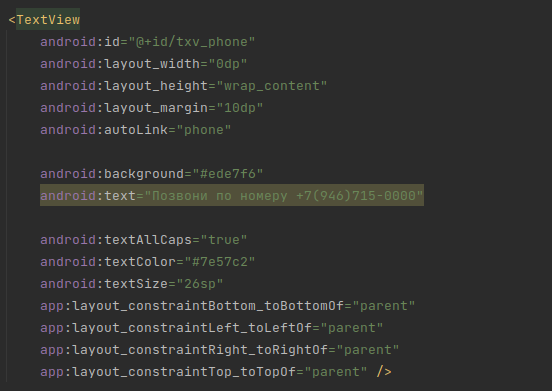
\includegraphics[width=0.8\textwidth]{Screenshot from 2023-03-23 10-28-13.png}
	\caption{Пример TextView}
	\label{fig:textview}
\end{figure}

\section{Элемент EditText}
Элемент EditText является подклассом класса TextView. Он также 
представляет текстовое поле, но теперь уже с возможностью ввода и 
редактирования текста. Таким образом, в EditText мы можем использовать 
все те же возможности, что и в TextView. Из тех атрибутов, что не 
рассматривались в теме про TextView, следует отметить атрибут android:hint. 
Он позволяет задать текст, который будет отображаться в качестве 
подсказки, если элемент EditText пуст. Кроме того, мы можем использовать 
атрибут \texttt{android:inputType}, который позволяет задать
клавиатуру для ввода.
Данный виджет проиллюстрирован на рисунке~\ref{fig:edittext}.

\begin{figure}[h!tp]
	\centering
	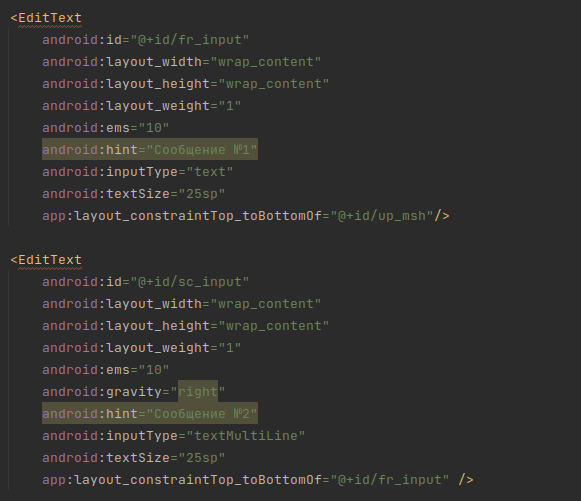
\includegraphics[width=0.9\textwidth]{Screenshot from 2023-03-23 10-31-28.png}
	\caption{Пример EditText}
	\label{fig:edittext}
\end{figure}

\section{Элемент Button}
Одним из часто используемых элементов являются кнопки, которые 
представлены классом android.widget.Button. Ключевой особенностью кнопок 
является возможность взаимодействия с пользователем через нажатия. 
Наследуется от класса TextView с новым методом \texttt{onClick}.
Данный виджет проиллюстрирован на рисунке~\ref{fig:button}.

\begin{figure}[h!tp]
	\centering
	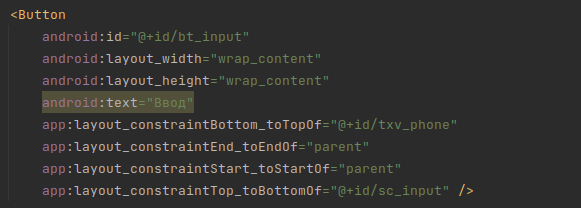
\includegraphics[width=0.9\textwidth]{Screenshot from 2023-03-23 10-36-14.png}
	\caption{Пример EditText}
	\label{fig:button}
\end{figure}

\section{Класс Toast}
Для создания простых уведомлений в Android используется класс 
Toast. Фактически Toast представляет всплывающее окно с некоторым 
текстом, которое отображается в течение некоторого времени. Объект Toast 
нельзя создать в коде разметки xml, например, в файлe activity\_main.xml. 
Toast можно использовать только в коде java.
Данный виджет проиллюстрирован на рисунке~\ref{fig:toast}.

\begin{figure}[h!tp]
	\centering
	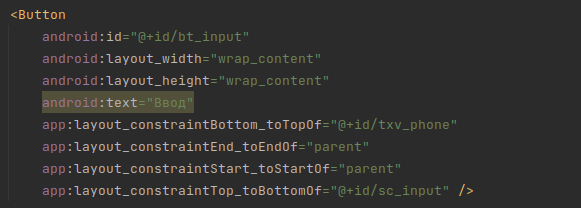
\includegraphics[width=0.9\textwidth]{Screenshot from 2023-03-23 10-36-14.png}
	\caption{Пример использования Toast}
	\label{fig:toast}
\end{figure}

\section{Элемент Snackbar}
Элемент Snackbar в некотором роде похож на Toast: он также позволяет 
выводить всплывающие сообщения, но теперь сообщения растягиваются по 
ширине экрана.
Данный виджет проиллюстрирован на рисунке~\ref{fig:snackbar}.

\begin{image}
	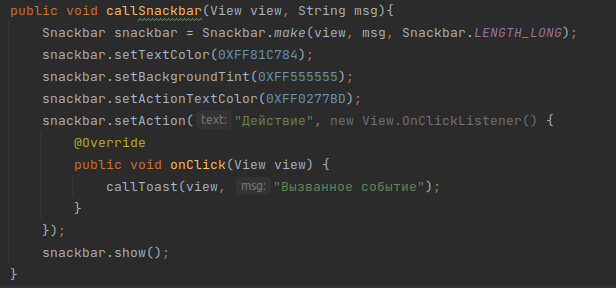
\includegraphics[width=0.8\textwidth]{Screenshot from 2023-03-25 17-11-35.png}
	\caption{Пример использования Snackbar}
	\label{fig:snackbar}
\end{image}

\section{Элементы Checkbox}
Элементы Checkbox представляют собой флажки, которые могут 
находиться в отмеченном и неотмеченном состоянии. Флажки позволяют 
производить множественный выбор из нескольких значений.
Данный виджет проиллюстрирован на рисунке~\ref{fig:checkbox}.

\begin{image}
	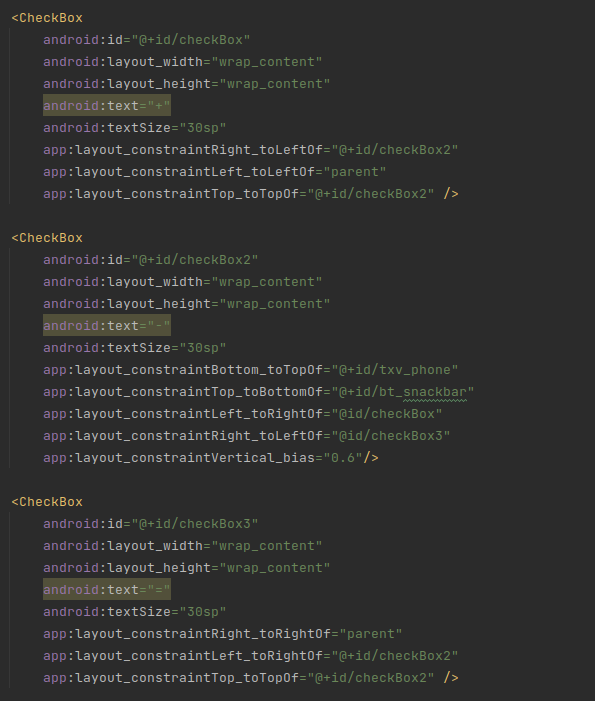
\includegraphics[width=0.8\textwidth]{Screenshot from 2023-03-25 17-25-07.png}
	\caption{Пример использования CheckBox}
	\label{fig:checkbox}
\end{image}

\section{Слушатель OnCheckedChangeListener}
Применение слушателя OnCheckedChangeListener представляет
альтернативный способ отслеживания изменения флажка. Этот слушатель 
срабатывает, когда устанавливается или убирается отметка на флажке.\par
Слушатель OnCheckedChangeListener определен в базовом классе
CompoundButton и определяет один метод --- \texttt{onCheckedChanged}. Первый
параметр этого метода \texttt{buttonView} --- сам измененный флажок CheckBox.
А второй параметр \texttt{isChecked} указывает, отмечен ли флажок.
Данный виджет проиллюстрирован на рисунке~\ref{fig:checkedchangelistener}.

\begin{image}
	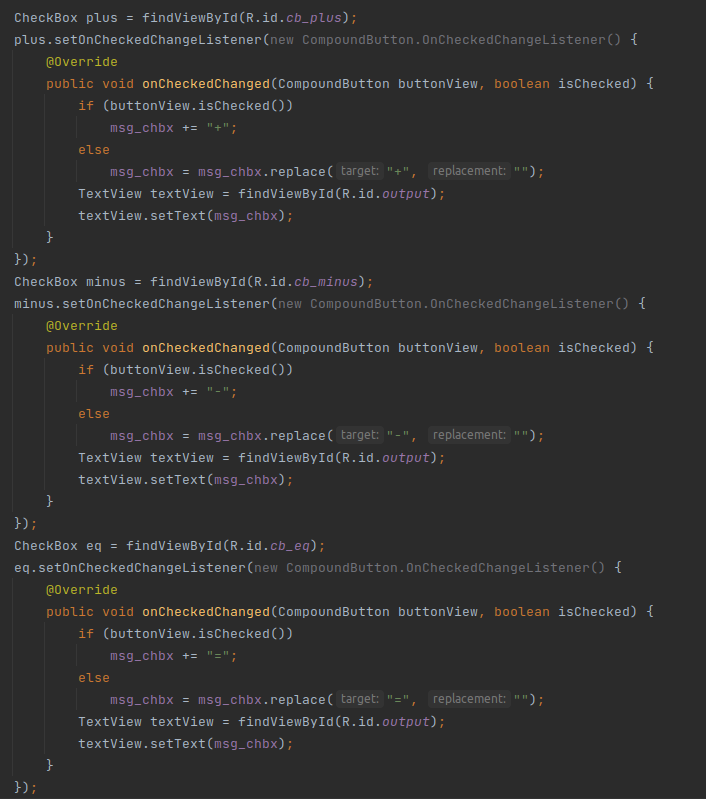
\includegraphics[width=0.8\textwidth]{Screenshot from 2023-03-25 17-51-18.png}
	\caption{Пример использования OnCheckedChangeListener}
	\label{fig:checkedchangelistener}
\end{image}

\section{Элемент ToggleButton}
ToggleButton подобно элементу CheckBox может пребывать в двух 
состояниях: отмеченном и неотмеченном, причем для каждого состояния мы 
можем отдельно установить свой текст.
Данный виджет проиллюстрирован на рисунке~\ref{fig:togglebutton}.

\begin{image}
	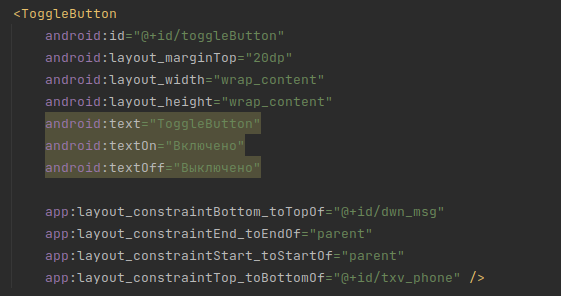
\includegraphics[width=0.8\textwidth]{Screenshot from 2023-03-25 17-55-50.png}
	\caption{Пример использования ToggleButton}
	\label{fig:togglebutton}
\end{image}

\section{Класс RadioButton}
Схожую с флажками функциональность предоставляют 
переключатели, которые представлены классом RadioButton. Но в отличие от 
флажков единовременно в группе переключателей мы можем выбрать только 
один переключатель. Чтобы создать список переключателей для выбора, 
вначале надо создать объект RadioGroup, который будет включать в себя все 
переключатели.
Данный виджет проиллюстрирован на рисунке~\ref{fig:radiobutton}.

\begin{image}
	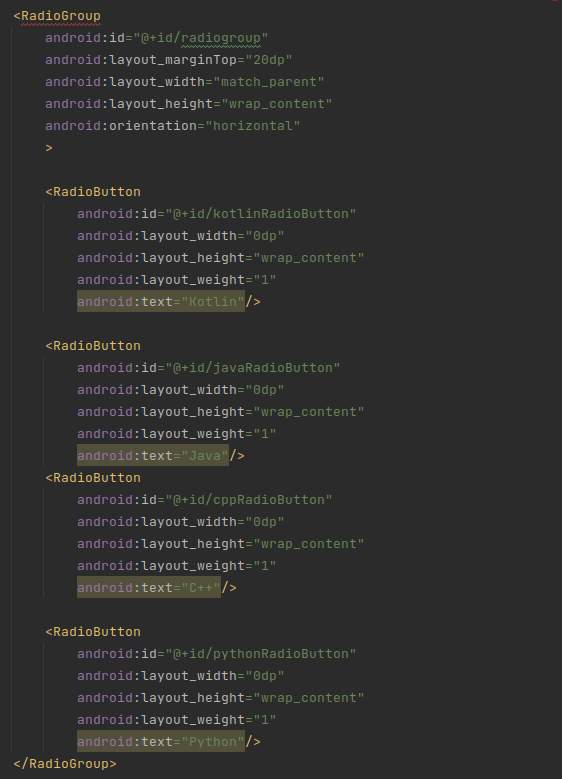
\includegraphics[width=0.8\textwidth]{Screenshot from 2023-03-25 18-03-35.png}
	\caption{Пример использования RadioGroup}
	\label{fig:radiobutton}
\end{image}

\section{Элемент DatePicker}

DatePicker представляет элемент для выбора даты. Среди его атрибутов 
можно отметить следующие:
\begin{itemize}
	\item \texttt{android:calendarTextColor}: цвет текста календаря;
	\item \texttt{android:calendarViewShown}: указывает, будет ли
		отображаться вид календаря;
	\item \texttt{android:datePickerMode}: устанавливает режим выбора даты;
	\item \texttt{android:dayOfWeekBackground}: устанавливает фоновый цвет
		панели выбора дня недели;
	\item \texttt{android:endYear}: устанавливает последний отображаемый год;
	\item \texttt{android:firstDayOfWeek}: устанавливает первый день недели;
	\item \texttt{android:headerBackground}: устанавливает фоновый цвет
		для панели выбранной даты;
	\item \texttt{android:maxDate}: устанавливает максимальную отображаемую
		дату в формате mm/dd/yyyy;
	\item \texttt{android:minDate}: устанавливает минимальную отображаемую
		дату в формате mm/dd/yyyy;
	\item \texttt{android:spinnersShown}: указывает, будет ли отображаться
		спиннер в виджете;
	\item \texttt{android:startYear}: устанавливает начальный
		отображаемый год;
	\item \texttt{android:yearListSelectorColor}: устанавливает цвет для
		поля выбора года.
\end{itemize}

Данный виджет проиллюстрирован на рисунке~\ref{fig:datepicker}.

\begin{image}
	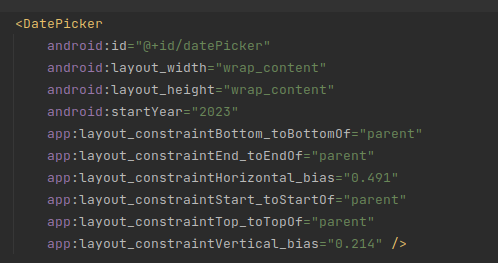
\includegraphics[width=0.8\textwidth]{Screenshot from 2023-03-25 18-07-26.png}
	\caption{Пример использования DatePicker}
	\label{fig:datepicker}
\end{image}

\section{Элемент TimePicker}
TimePicker представляет виджет для выбора времени, который может 
отображать время либо в 24-часовом, либо в 12-часовом формате. Среди 
атрибутов TimePicker следует выделить \texttt{timePickerMode},
который позволяет режим отображения и может принимать одно из двух значений:
\texttt{clock} (отображение в виде часов) и
\texttt{spinner} (отображение в виде спиннера).
Среди методов TimePicker можно отметить следующие:

\begin{itemize}
	\item \texttt{int getHour()}: возвращает час (в 24-часом формате);
	\item \texttt{int getMinute()}: возвращает минуты;
	\item \texttt{boolean is24HourView()}: возвращает true, если
		используется 24- часовой формат;
	\item \texttt{void setHour(int hour)}: устанавливает час для TimePicker;
	\item \texttt{void setIs24HourView(Boolean is24HourView)}:
		устанавливает 24- часовой формат;
	\item \texttt{void setMinute(int minute)}: устанавливает минуты;
	\item \texttt{void setOnTimeChangedListener(TimePicker.OnTimeChangedListener 
		onTimeChangedListener)}: устанавливает слушатель изменения времени 
		в TimePicker в виде объекта.
\end{itemize}

Данный виджет проиллюстрирован на рисунке~\ref{fig:timepicker}.

\begin{image}
	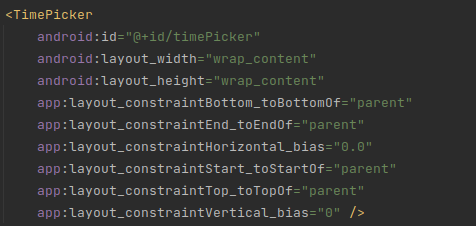
\includegraphics[width=0.8\textwidth]{Screenshot from 2023-03-25 18-09-56.png}
	\caption{Пример использования TimePicker}
	\label{fig:timepicker}
\end{image}

\section{Элемент SeekBar (Ползунок)}
Элемент SeekBar выполняет роль ползунка, то есть шкалу делений, на 
которой мы можем менять текущую отметку. Среди его атрибутов можно 
отметить следующие:

\begin{itemize}
	\item \texttt{android:max}: устанавливает максимальное значение;
	\item \texttt{android:min}: устанавливает минимальное значение;
	\item \texttt{android:progress}: устанавливает текущее значение,
		которое находится в диапазоне между минимальным и максимальным.
\end{itemize}

Данный виджет проиллюстрирован на рисунке~\ref{fig:seekbar}.

\begin{image}
	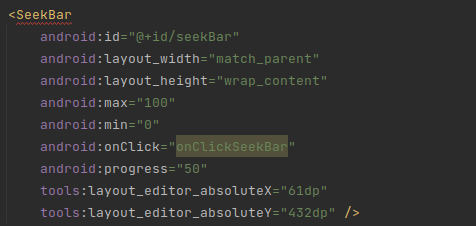
\includegraphics[width=0.8\textwidth]{Screenshot from 2023-03-25 18-11-54.png}
	\caption{Пример использования SeekBar}
	\label{fig:seekbar}
\end{image}


\clearpage

\section*{\LARGE{Вывод}}
\addcontentsline{toc}{section}{Вывод}
В ходе проделанной практической работы были получены навыки и 
знания с работой TextView, EditView, Button, Toast, Snackbar, CheckBox, 
ToggleButton, RadioButton/RadioGroup, TimePicker, DatePicker, Seekbar.

